\scanpage{6}
\mspage{4}
$\unsure{u_{2n-i}|\pi_{2n-i}}$ est \unsure{donc} la \deleted{\unsure{qui}} conjonction des suivantes :
\[
\begin{array}{l}(3.1.)_i\\[18pt](3.2)_i\end{array}
\quad\left.\begin{array}{l}\Bigl[
\bigl(u\in\unsure{\mathfrak Z|\mathcal Z}\mathcal E^0,\ \deleted{\unsure{\pi_\alpha u=0\ (\alpha\neq i),}}\ 
\figure{\begin{tikzpicture}[baseline=(e.base)]\node[draw,ellipse,inner sep=2pt] (e) {$\mathcal E_i^{2n-i}$};\end{tikzpicture}}u=0\bigr)
\Longrightarrow\deleted{u=0}\inserted{\pi_i u=0},\\[12pt]
\bigl(u\in\unsure{\mathfrak Z|\mathcal Z}\mathcal E^0,\ \deleted{\unsure{\pi_\alpha u=0\ (\alpha\neq2n-i),}}\ u\mathcal E_i^{2n-i}=0\bigr)
\Longrightarrow\deleted{u=0}\inserted{\pi_{2n-i}u=0}
\end{array}\right]
\]
En effet, la relation $(3.1.)$ implique que \deleted{$\unsure{\pi_i(\mathfrak Z\mathcal E^0)}$}\inserted{l'annulateur de $\pi_i$ dans $\unsure{\mathfrak Z|\mathcal Z}\mathcal E^0$} est l'idéal des $u\in\unsure{\mathfrak Z|\mathcal Z}\mathcal E^0$ tels que $\mathcal E_i^{2n-i}u=0$; or dans un anneau commutatif, un idempotent est connu quand on connaît son annulateur. De même pour $\pi_{2n-i}$, son annulateur dans $\unsure{\mathfrak Z|\mathcal Z}\mathcal E^0$ est formé des $u\in\unsure{\mathfrak Z|\mathcal Z}\mathcal E^0$ tels que $u\mathcal E_i^{2n-i}=0$.

En même temps, les conditions $(3.1.)_i$, $(3.2.)_i$ pour tt $i$, donnent un \deleted{condition} procédé pour déterminer de proche en proche les $\pi_i$.

\figure{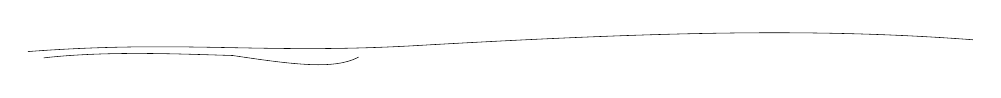
\begin{tikzpicture}[x=1cm,y=1cm]\draw[line width=.2pt] (0,0) .. controls (2,.15) and (3,-.04) .. (5,.08) .. controls (8,.25) and (10,.30) .. (12,.15);\draw[line width=.2pt] (.2,-.08) .. controls (1,.01) and (1.9,-.03) .. (2.6,-.05) .. controls (3.4,-.17) and (3.9,-.23) .. (4.2,-.07);\end{tikzpicture}}

4. Lorsque $\mathcal E^*$ est comme dans 1., une condition suffisante pour avoir $(3.1)_i$ \inserted{resp. $(3.2)_i$} est la \deleted{\unsure{suff}} suivante

$(\unsure{4.1})_i$ L'intersection des noyaux des $v:M^i\longrightarrow M^{2n-i}$, pour $v\in\mathcal E_i^{2n-i}$, est réduite à $0$.

$(4.2)_i$ La somme des images des $v:M^i\unsure{-|\longrightarrow}M^{2n-i}$, pour $v\in\mathcal E_i^{2n-i}$, est \deleted{\unsure{à}} égale à $M^{2n-i}$.

Ces deux conditions sont satisfaites si on a

$(4.3)_i$ Il existe \inserted{$v:M^i\unsure{-|\longrightarrow}M^{2n-i}$,} $v\in\mathcal E_i^{2n-i}$, qui est un isom. de
\mspage{5}
